\graphicspath{{chapters/04/media/}}
\chapter{Analisi dei dati}
\label{cha:analisi}
%  \begin{figure}[H]
%    \centering
%    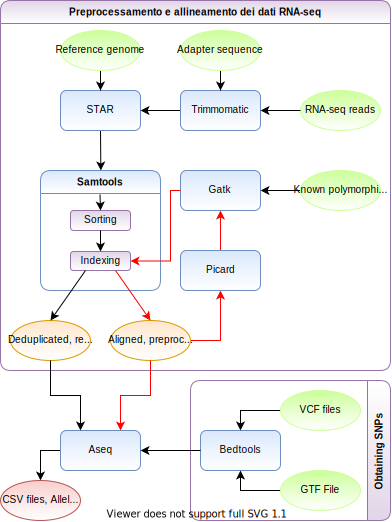
\includegraphics[scale=0.2]{pipeline.png}
%    \caption{Pipeline per l'ottenimento dei dati di allelic imbalance}
%    \label{fig:}
%  \end{figure}

\section{Identificazione delle varianti}

 \begin{figure}[H]
   \centering
   \includegraphics[scale=1]{scelta_gtf.png}
   \caption{SNP mantenuti dopo l'intersezione con i VCF}
   \label{fig:}
 \end{figure}

\section{Conta degli SNP trovati con ASEQ}
\label{sec:snp_count}
 \begin{figure}[H]
   \centering
   \includegraphics[scale=1]{aseq_count_2_8_10_pre.png}
	 \caption{Conta per campione degli SNP eterozigoti trovati con aseq ($0.2< af < 0.8$ e coverage $\ge 10$)}
   \label{fig:}
 \end{figure}

 \subsection{Distrubuzione degli SNP}
 \begin{figure}[H]
   \centering
   \begin{tabular}{ccc}
      \subfloat[scr DMSO]{\includegraphics[width = 0.3\textwidth]{distribution/scr_DMSO.png}} &
      \subfloat[scr NUTLIN]{\includegraphics[width = 0.3\textwidth]{distribution/scr_NUTLIN.png}} &
      \subfloat[shDHX30 DMSO]{\includegraphics[width = 0.3\textwidth]{distribution/shDHX30_DMSO.png}} \\
      \subfloat[shDHX30 NUTLIN]{\includegraphics[width = 0.3\textwidth]{distribution/shDHX30_NUTLIN.png}} &
      \subfloat[shPCBP2 DMSO]{\includegraphics[width = 0.3\textwidth]{distribution/shPCBP2_DMSO.png}} &
      \subfloat[shPCBP2 NUTLIN]{\includegraphics[width = 0.3\textwidth]{distribution/shPCBP2_NUTLIN.png}} \\
  \end{tabular}
   \label{fig:}
 \end{figure}

\section{Qualit\`a dei campioni}
Confronto tra replicato di un campione in modo da verificare come cambiano i valori di AF tra un replicato e l'altro.
 \begin{figure}[H]
   \centering
   \begin{tabular}{ccc}
      \subfloat[1 - 2]{\includegraphics[width = 0.3\textwidth]{rep_corr/scr_DMSO_TOT-rep-1-2.post.0.2.0.8.10.png}} &
      \subfloat[1 - 3]{\includegraphics[width = 0.3\textwidth]{rep_corr/scr_DMSO_TOT-rep-1-3.post.0.2.0.8.10.png}} &
      \subfloat[1 - 4]{\includegraphics[width = 0.3\textwidth]{rep_corr/scr_DMSO_TOT-rep-1-4.post.0.2.0.8.10.png}} \\
      \subfloat[2 - 3]{\includegraphics[width = 0.3\textwidth]{rep_corr/scr_DMSO_TOT-rep-2-3.post.0.2.0.8.10.png}} &
      \subfloat[2 - 4]{\includegraphics[width = 0.3\textwidth]{rep_corr/scr_DMSO_TOT-rep-2-4.post.0.2.0.8.10.png}} &
      \subfloat[3 - 4]{\includegraphics[width = 0.3\textwidth]{rep_corr/scr_DMSO_TOT-rep-3-4.post.0.2.0.8.10.png}} \\
  \end{tabular}
   \label{fig:}
 \end{figure}

\section{Considerazioni sulla recalibrazione}
\label{sec:rec_cons}
Discussione dei risultati di ASEQ prima e dopo la recalibrazione.
 \begin{figure}[H]
   \centering
   \begin{tabular}{ccc}
      \subfloat[scr DMSO polisomale]{\includegraphics[width = 0.3\textwidth]{correlation_recal/scr_DMSO_POL_1.png}} &
      \subfloat[scr DMSO totale]{\includegraphics[width = 0.3\textwidth]{correlation_recal/scr_DMSO_TOT_1.png}} &
      \subfloat[scr NUTLIN polisomale]{\includegraphics[width = 0.3\textwidth]{correlation_recal/scr_NUTLIN_POL_1.png}} \\
      \subfloat[scr NUTLIN totale]{\includegraphics[width = 0.3\textwidth]{correlation_recal/scr_NUTLIN_TOT_1.png}} &
      \subfloat[shDHX30 DMSO polisomale]{\includegraphics[width = 0.3\textwidth]{correlation_recal/shDHX30_DMSO_POL_1.png}} &
      \subfloat[shDHX30 DMSO totale]{\includegraphics[width = 0.3\textwidth]{correlation_recal/shDHX30_DMSO_TOT_1.png}} \\
      \subfloat[shDHX30 NUTLIN polisomale]{\includegraphics[width = 0.3\textwidth]{correlation_recal/shDHX30_NUTLIN_POL_1.png}} &
      \subfloat[shDHX30 NUTLIN totale]{\includegraphics[width = 0.3\textwidth]{correlation_recal/shDHX30_NUTLIN_TOT_1.png}} &
      \subfloat[shPCBP2 DMSO polisomale]{\includegraphics[width = 0.3\textwidth]{correlation_recal/shPCBP2_DMSO_POL_1.png}} \\
      \subfloat[shPCBP2 DMSO totale]{\includegraphics[width = 0.3\textwidth]{correlation_recal/shPCBP2_DMSO_TOT_1.png}} &
      \subfloat[shPCBP2 NUTLIN polisomale]{\includegraphics[width = 0.3\textwidth]{correlation_recal/shPCBP2_NUTLIN_POL_1.png}} &
      \subfloat[shPCBP2 NUTLIN totale]{\includegraphics[width = 0.3\textwidth]{correlation_recal/shPCBP2_NUTLIN_TOT_1.png}} \\
  \end{tabular}
   \label{fig:}
 \end{figure}

\section{Ottenere i dati per gli SNP di interesse}
\label{sec:snp_filter}
Discussione degli SNP con i dati necessari per lo studio e scelta degli SNP di interesse.
Ovvero come \`e stata ottenuta la lista da cellminer, i t-test.
Magari qua posso mettere un barplot con la conta degli SNP trovati.

   \subsection{Boxplot}
   I boxplot degli SNP trovati.
 \begin{figure}[H]
   \centering
   \begin{tabular}{cc}
      \subfloat[scr DMSO rs1131941]{\includegraphics[width = 0.5\textwidth]{boxplot/scr_DMSO_rs1131941.png}} &
      \subfloat[scr DMSO rs2228626]{\includegraphics[width = 0.5\textwidth]{boxplot/scr_DMSO_rs2228626.png}} \\
      \subfloat[scr DMSO rs2289373]{\includegraphics[width = 0.5\textwidth]{boxplot/scr_DMSO_rs2289373.png}} &
      \subfloat[shPCBP2 NUTLIN rs9833]{\includegraphics[width = 0.5\textwidth]{boxplot/shPCBP2_NUTLIN_rs9833.png}} \\
  \end{tabular}
   \label{fig:}
 \end{figure}

\section{Caratterizzazione degli SNP di interesse}
Magari una lista contenente gli SNP caratterizzati con snpEff




\section{Conclusioni}
\label{sec:ending}
